\documentclass[conference]{IEEEtran}
\usepackage{amsmath,amssymb}
\usepackage{graphicx}
\usepackage{booktabs}
\usepackage{tikz}
\usetikzlibrary{positioning,arrows.meta}
\usepackage{listings}
\usepackage{url}
\usepackage{cite}
\newcommand{\dsRatings}{\textbf{--}}
\newcommand{\dsUsers}{\textbf{--}}
\newcommand{\dsItems}{\textbf{--}}
\newcommand{\ingestSec}{\textbf{--}}
\newcommand{\nTrain}{\textbf{--}}
\newcommand{\nVal}{\textbf{--}}
\newcommand{\nTest}{\textbf{--}}
\newcommand{\rmseGlobal}{\textbf{--}}
\newcommand{\rmseItem}{\textbf{--}}
\newcommand{\rmseAls}{\textbf{--}}
\newcommand{\bestRank}{\textbf{--}}
\newcommand{\bestReg}{\textbf{--}}
\newcommand{\alsFitSec}{\textbf{--}}
\newcommand{\alsCoverage}{\textbf{--}}
\newcommand{\evalUsers}{\textbf{--}}
\newcommand{\precPop}{\textbf{--}}
\newcommand{\precAls}{\textbf{--}}
\newcommand{\recPop}{\textbf{--}}
\newcommand{\recAls}{\textbf{--}}
\newcommand{\covPop}{\textbf{--}}
\newcommand{\covAls}{\textbf{--}}
\newcommand{\churnUsers}{\textbf{--}}
\newcommand{\churnRate}{\textbf{--}}
\newcommand{\aucLR}{\textbf{--}}
\newcommand{\aucGBT}{\textbf{--}}
\newcommand{\prLR}{\textbf{--}}
\newcommand{\prGBT}{\textbf{--}}
\newcommand{\topFeatA}{\textbf{--}}
\newcommand{\topFeatB}{\textbf{--}}
\newcommand{\topFeatC}{\textbf{--}}
\newcommand{\streamRows}{\textbf{--}}
   % auto-generated by src/make_paper_assets.py from results/*.json
\lstset{basicstyle=\ttfamily\scriptsize,frame=single,breaklines=true,columns=fullflexible}

\begin{document}
\title{Scalable OTT Recommendation and\\Churn-Signal Detection with Apache Spark}

\author{\IEEEauthorblockN{[Author 1 Name]}
\IEEEauthorblockA{Dept.\ of Computer Engineering\\Vidyalankar Institute of Technology, Mumbai, India\\
email1@vit.edu.in}
\and
\IEEEauthorblockN{[Author 2 Name]}
\IEEEauthorblockA{Dept.\ of Computer Engineering\\Vidyalankar Institute of Technology, Mumbai, India\\
email2@vit.edu.in}}
\maketitle

\begin{abstract}
Over-the-top (OTT) streaming platforms depend on recommendation engines to keep viewers engaged, and on early detection of disengagement to reduce subscriber churn. Both tasks operate on very large, sparse and continuously growing interaction logs. We present an end-to-end Big Data pipeline built on Apache Spark that (i) ingests the MovieLens 25M ratings corpus into columnar storage, (ii) trains a distributed Alternating Least Squares (ALS) collaborative-filtering model with a leak-free chronological split, (iii) derives an engagement-decay churn signal from behavioural features, and (iv) demonstrates low-latency serving with Spark Structured Streaming. The tuned ALS model attains a test RMSE of \rmseAls{} against \rmseGlobal{} for a global-mean baseline, and a Precision@10 of \precAls{} versus \precPop{} for a popularity baseline. A gradient-boosted churn classifier reaches an ROC-AUC of \aucGBT{}. All code and instructions are publicly available.
\end{abstract}

\begin{IEEEkeywords}
Big Data, Apache Spark, OTT analytics, collaborative filtering, ALS, churn prediction
\end{IEEEkeywords}

\section{Introduction}
Subscription video platforms compete on retention. Industry accounts of large OTT services report that personalised recommendation is central to how viewers find content and therefore to the value of the service~\cite{netflix}. A viewer who cannot quickly find something to watch is more likely to disengage, and sustained disengagement is the strongest precursor of cancellation.

The underlying data is a textbook Big Data workload. Interaction logs reach billions of events; the user--item matrix is extremely sparse; new events arrive continuously; and the quality of the signal is uneven because popular titles dominate. Single-node tools struggle with the joins, shuffles and iterative factorisation that these workloads require, which motivates distributed engines such as Apache Spark~\cite{spark,mllib}.

\textbf{Contributions.} (1) A reproducible Spark pipeline from raw CSV to ranked recommendations, with all stages scripted. (2) A rigorous evaluation protocol that uses a chronological split, a rating-and-ranking metric suite and catalogue coverage. (3) An engagement-decay churn signal computed strictly from pre-cutoff behaviour. (4) A streaming serving demonstration that illustrates the velocity dimension of the problem.

\section{Related Work}
Matrix factorisation is the dominant family of collaborative-filtering methods since the Netflix Prize~\cite{koren}. For implicit and explicit feedback, Hu et al.\ introduced a confidence-weighted least-squares formulation~\cite{hu}, and Zhou et al.\ showed that alternating least squares parallelises naturally across machines~\cite{zhou}, which is the basis of Spark MLlib's implementation~\cite{mllib}. Gradient boosting~\cite{friedman} is a standard strong baseline for tabular behavioural prediction such as churn. Spark Structured Streaming~\cite{structured} extends the same DataFrame API to unbounded data. We combine these established components into a single OTT-oriented pipeline and focus on evaluation hygiene (time-aware splitting, cold-start handling and ranking metrics) rather than on a new algorithm.

\section{Dataset and Problem Formulation}
We use the MovieLens 25M dataset~\cite{movielens}, which contains \dsRatings{} ratings from \dsUsers{} users on \dsItems{} movies, each with a 0.5--5.0 star score and a timestamp. We use it as a public proxy for OTT viewing feedback.

\textbf{Task A (recommendation).} Given a user's history up to time $t$, rank unseen titles. Predicted ratings are scored by RMSE; ranked lists by Precision@$K$ and Recall@$K$ with $K{=}10$, treating ratings $\ge 4$ as relevant.

\textbf{Task B (churn signal).} Let $t_c$ be the 80th percentile of event time. A user with at least five events before $t_c$ is labelled \emph{churned} if they produce no events after $t_c$. This is a disengagement proxy, because the dataset has no subscription cancellations; it should be read as an engagement signal and not as true billing churn.

\subsection{Evaluation metrics}
For a test set $T$ of ratings, $\mathrm{RMSE}=\sqrt{|T|^{-1}\sum_{(u,i)\in T}(r_{ui}-\hat r_{ui})^2}$. For user $u$ with ranked list $L_u^{K}$ and relevant set $\mathcal{R}_u$,
\begin{equation}
\mathrm{P@}K=\frac{|L_u^{K}\cap\mathcal{R}_u|}{K},\quad \mathrm{R@}K=\frac{|L_u^{K}\cap\mathcal{R}_u|}{|\mathcal{R}_u|},
\end{equation}
averaged over users. Catalogue coverage is $|\bigcup_u L_u^{K}|/|\mathcal{I}|$, where $\mathcal{I}$ is the set of titles. For churn we report ROC-AUC and PR-AUC, because the positive class can be imbalanced.

\subsection{Big Data characteristics}
\begin{table}[t]
\caption{Mapping of the five Vs to this OTT workload.}
\label{tab:vs}
\centering
\small
\begin{tabular}{lp{5.2cm}}
\toprule
Characteristic & In this project \\
\midrule
Volume & Millions of ratings; user--item matrix with $\gg$99\% missing entries \\
Velocity & Continuous viewing events; simulated via Structured Streaming \\
Variety & Ratings, timestamps, multi-valued genre strings \\
Veracity & Popularity bias, self-selected raters, sparse users/items \\
Value & Better discovery and earlier detection of disengagement \\
\bottomrule
\end{tabular}
\end{table}

\section{System Architecture}
Fig.~\ref{fig:arch} shows the pipeline. Each stage is a separate Spark job that reads and writes Parquet, so stages can be rerun independently.

\begin{figure*}[t]
\centering
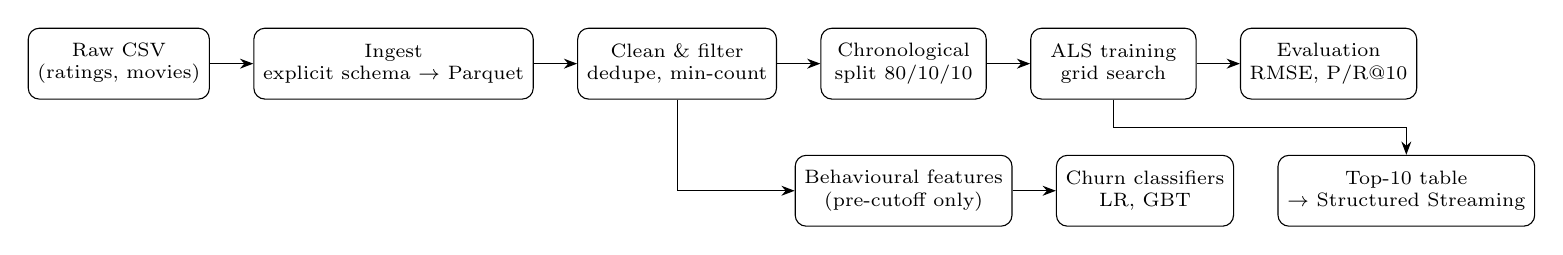
\begin{tikzpicture}[node distance=0.55cm, box/.style={draw,rounded corners,minimum height=0.9cm,minimum width=2.1cm,align=center,font=\scriptsize}, >=Stealth]
\node[box] (a) {Raw CSV\\(ratings, movies)};
\node[box,right=of a] (b) {Ingest\\explicit schema $\to$ Parquet};
\node[box,right=of b] (c) {Clean \& filter\\dedupe, min-count};
\node[box,right=of c] (d) {Chronological\\split 80/10/10};
\node[box,right=of d] (e) {ALS training\\grid search};
\node[box,right=of e] (f) {Evaluation\\RMSE, P/R@10};
\node[box,below=0.7cm of d] (g) {Behavioural features\\(pre-cutoff only)};
\node[box,right=of g] (h) {Churn classifiers\\LR, GBT};
\node[box,right=of h] (i) {Top-10 table\\$\to$ Structured Streaming};
\foreach \x/\y in {a/b,b/c,c/d,d/e,e/f,g/h} \draw[->] (\x)--(\y);
\draw[->] (c.south) |- (g.west);
\draw[->] (e.south) -- ++(0,-0.35) -| (i.north);
\end{tikzpicture}
\caption{End-to-end pipeline. Every arrow is a Parquet hand-off between independent Spark jobs.}
\label{fig:arch}
\end{figure*}

\subsection{Ingestion and cleaning}
CSVs are read with explicit schemas, which avoids a schema-inference pass over the data, then de-duplicated on $(user,item)$ and written as Parquet. Ingestion took \ingestSec{} s on our machine. Users and items with fewer than five ratings are removed to limit extreme sparsity; remaining cold-start cases in the test period are handled in Section~\ref{sec:eval}.

\subsection{Chronological split}
A random split would let the model train on events that happen after test events. We instead split on global timestamp quantiles: the earliest 80\% for training (\nTrain{} rows), the next 10\% for validation (\nVal{}) and the final 10\% for testing (\nTest{}).

\subsection{ALS model}
ALS approximates the rating matrix $R\in\mathbb{R}^{m\times n}$ as $R\approx UV^{\top}$ with $U\in\mathbb{R}^{m\times k}$, $V\in\mathbb{R}^{n\times k}$, minimising
\begin{equation}
\sum_{(u,i)\in\Omega}\!\left(r_{ui}-\mathbf{u}_u^{\top}\mathbf{v}_i\right)^2+\lambda\Big(\sum_u\lVert\mathbf{u}_u\rVert^2+\sum_i\lVert\mathbf{v}_i\rVert^2\Big).
\end{equation}
Fixing $V$ makes the problem a set of independent per-user least-squares solves, and vice versa, so each half-step is embarrassingly parallel across partitions~\cite{zhou,mllib}. The core of the implementation is shown below.
\begin{lstlisting}[language=Python]
als = ALS(userCol="userId", itemCol="movieId",
          ratingCol="rating", rank=k, regParam=lam,
          maxIter=10, nonnegative=True,
          coldStartStrategy="drop", seed=42)
model = als.fit(train_plus_val)
recs = model.recommendForUserSubset(users, 200)
\end{lstlisting}
We grid-search rank $k$ and regularisation $\lambda$ on the validation split, then retrain on train+validation with the best setting and score the held-out test period. We use non-negative factors and \texttt{coldStartStrategy=drop}.

\subsection{Churn features and models}
\begin{table}[t]
\caption{Behavioural features used for churn prediction (all computed before $t_c$).}
\label{tab:feat}
\centering
\small
\begin{tabular}{ll}
\toprule
Feature & Meaning \\
\midrule
\texttt{n\_ratings}, \texttt{n\_titles} & Event count; distinct titles \\
\texttt{avg\_rating}, \texttt{std\_rating} & Mean and spread of scores \\
\texttt{n\_genres} & Genre diversity \\
\texttt{span\_days} & First-to-last event interval \\
\texttt{days\_since\_last} & Recency of last event \\
\texttt{r\_last30}, \texttt{r\_last90} & Events in last 30/90 days \\
\texttt{recent\_ratio} & \texttt{r\_last90}/\texttt{n\_ratings} \\
\bottomrule
\end{tabular}
\end{table}
Features are computed strictly from events before $t_c$: rating count, mean and standard deviation of ratings, distinct titles, genre diversity, activity span, days since last event, and counts in the last 30 and 90 days (with their ratio to total activity). We compare logistic regression with a gradient-boosted tree classifier~\cite{friedman} on a random 80/20 user split.

\subsection{Streaming serving}
The final top-10 lists are stored as a table. A rate-source stream of synthetic viewing events is joined with that table inside Spark Structured Streaming~\cite{structured} with 2-second micro-batches, simulating on-demand recommendation lookups. In a 15-second test it served \streamRows{} lists. This demonstrates the serving pattern rather than production latency.

\section{Experimental Setup}\label{sec:eval}
All jobs ran in Spark local mode with PySpark. Hyper-parameters were rank $\in\{10,20,50\}$ and $\lambda\in\{0.05,0.1,0.2\}$ with 10 iterations. \textbf{Cold start:} test rows whose user or item is absent from training are dropped by ALS; we report the scored share as coverage (\alsCoverage\%). \textbf{Ranking evaluation:} for a random sample of \evalUsers{} test users with at least one relevant item, we request 200 candidates from ALS, remove titles the user has already rated in train+validation, and keep the top 10. The popularity baseline recommends the most-rated unseen titles. We also report \emph{catalogue coverage}, the share of all titles that appear in any recommended list, as a proxy for diversity.

\begin{table}[t]
\caption{Experimental environment and configuration.}
\label{tab:env}
\centering
\small
\begin{tabular}{ll}
\toprule
Item & Value \\
\midrule
Hardware & [CPU model, cores, RAM] \\
Software & Spark 4.x (PySpark), Python 3.12 \\
Mode / driver memory & local[*] / [e.g.\ 8\,GB] \\
ALS grid & rank $\{10,20,50\}$, $\lambda\{0.05,0.1,0.2\}$ \\
ALS iterations / seed & 10 / 42 \\
Shuffle partitions & 64 \\
Relevance threshold & rating $\ge 4.0$ \\
\bottomrule
\end{tabular}
\end{table}

\textbf{Reproducibility.} The repository provides one script per stage and a wrapper (\texttt{run\_all.sh}) that downloads the data, runs every stage, and regenerates the numeric macros and figure used in this paper, so each table entry traces to a JSON file under \texttt{results/}.

\section{Results}
\subsection{Rating prediction}
\begin{table}[t]
\caption{Rating prediction on the chronological test set (lower is better).}
\label{tab:rmse}
\centering
\begin{tabular}{lc}
\toprule
Model & RMSE \\
\midrule
Global mean & \rmseGlobal \\
Item mean & \rmseItem \\
ALS (rank=\bestRank, $\lambda$=\bestReg) & \rmseAls \\
\bottomrule
\end{tabular}
\end{table}
Table~\ref{tab:rmse} compares ALS with two non-personalised baselines. The grid-search validation curve is shown in Fig.~\ref{fig:rank}. The final ALS fit on train+validation took \alsFitSec{} s.

\begin{figure}[t]
\centering
\IfFileExists{fig_rank.pdf}{\includegraphics[width=0.85\columnwidth]{fig_rank.pdf}}{\fbox{\parbox{0.8\columnwidth}{\centering\small Figure is generated by \texttt{make\_paper\_assets.py} after the experiments are run.}}}
\caption{Validation RMSE versus latent rank for each regularisation value.}
\label{fig:rank}
\end{figure}

\subsection{Top-10 ranking quality}
\begin{table}[t]
\caption{Top-10 recommendation quality on \evalUsers{} sampled test users.}
\label{tab:rank}
\centering
\begin{tabular}{lccc}
\toprule
Model & P@10 & R@10 & Catalogue cov.\ (\%) \\
\midrule
Popularity & \precPop & \recPop & \covPop \\
ALS & \precAls & \recAls & \covAls \\
\bottomrule
\end{tabular}
\end{table}
Table~\ref{tab:rank} reports ranking metrics. Because relevance is defined by the future test window and already-seen titles are excluded, absolute precision values are low by construction; the relative comparison between methods is what matters. % EDIT: adjust the next sentence to match the numbers you obtain.
Catalogue coverage indicates how much of the catalogue each method surfaces; popularity concentrates on a small head of titles.

\subsection{Churn signal}
\begin{table}[t]
\caption{Disengagement prediction on held-out users (\churnUsers{} users, \churnRate\% labelled churned).}
\label{tab:churn}
\centering
\begin{tabular}{lcc}
\toprule
Model & ROC-AUC & PR-AUC \\
\midrule
Logistic regression & \aucLR & \prLR \\
Gradient-boosted trees & \aucGBT & \prGBT \\
\bottomrule
\end{tabular}
\end{table}
Table~\ref{tab:churn} lists classifier performance. The most important GBT features were \texttt{\topFeatA}, \texttt{\topFeatB} and \texttt{\topFeatC}. % EDIT: interpret feature importance for your run.

\section{Discussion}
\textbf{Scalability.} Parquet storage with explicit schemas and a single shared Spark session per stage keep ingestion and feature computation inexpensive, and the ALS half-steps parallelise across partitions. Moving from local mode to a cluster requires only changing the master URL and partition counts.

\textbf{Threats to validity.} (i) Ratings are explicit feedback, whereas real platforms mostly observe implicit signals such as watch time. (ii) The churn label is an activity proxy, not a billing event. (iii) MovieLens users chose to rate, so selection bias exists. (iv) The streaming demo uses synthetic events. (v) Results come from a single run with a fixed seed; we did not compute confidence intervals.

\textbf{Complexity.} Each ALS iteration performs two sets of $k\times k$ normal-equation solves, costing roughly $O\big(|\Omega|k^{2}+(m+n)k^{3}\big)$ per iteration, plus shuffle traffic proportional to $|\Omega|k$. Rank therefore trades accuracy against both compute and network cost, which is why the grid search records fit time alongside validation RMSE.

\textbf{Cold start and fairness of evaluation.} Dropping unseen users and titles at test time flatters RMSE slightly because the hardest rows are excluded; we therefore report the scored share. A production system would route such rows to a content-based or popularity fallback.

\textbf{Practical implications.} A recommender is only useful if it exposes more of the catalogue than a popularity list while remaining accurate; reporting coverage next to accuracy makes that trade-off visible. The churn features are cheap to refresh and can feed retention actions such as personalised rows or re-engagement messages.

\section{Conclusion and Future Work}
We built and evaluated an open Spark pipeline for OTT recommendation and engagement-decay detection. Future work includes implicit-feedback ALS on watch-time data, a two-tower neural retrieval model, a feature store with Kafka ingestion for true streaming, and evaluation on data with real subscription outcomes.

\textbf{Ethical considerations.} Recommenders can reinforce popularity bias and narrow what users see. Reporting catalogue coverage is one safeguard; periodic audits of exposure by genre and release year are another. MovieLens contains no personal identifiers beyond anonymised user IDs, and no scraping or private data were used.

\section*{Contribution Statement}
\textbf{[Author 1]:} data ingestion, cleaning, chronological split, churn features, repository and README. \textbf{[Author 2]:} ALS modelling, hyper-parameter search, evaluation metrics, streaming demo and figures. Both authors designed the architecture and wrote and reviewed the paper.

\section*{Code Availability}
Code, run scripts and instructions: \url{https://github.com/[username]/ott-bigdata-pipeline}.

\begin{thebibliography}{10}
\bibitem{movielens} F. M. Harper and J. A. Konstan, ``The MovieLens datasets: History and context,'' \emph{ACM Trans. Interact. Intell. Syst.}, vol. 5, no. 4, pp. 1--19, 2015.
\bibitem{spark} M. Zaharia \emph{et al.}, ``Apache Spark: A unified engine for big data processing,'' \emph{Commun. ACM}, vol. 59, no. 11, pp. 56--65, 2016.
\bibitem{mllib} X. Meng \emph{et al.}, ``MLlib: Machine learning in Apache Spark,'' \emph{J. Mach. Learn. Res.}, vol. 17, no. 34, pp. 1--7, 2016.
\bibitem{koren} Y. Koren, R. Bell, and C. Volinsky, ``Matrix factorization techniques for recommender systems,'' \emph{Computer}, vol. 42, no. 8, pp. 30--37, 2009.
\bibitem{hu} Y. Hu, Y. Koren, and C. Volinsky, ``Collaborative filtering for implicit feedback datasets,'' in \emph{Proc. IEEE ICDM}, 2008, pp. 263--272.
\bibitem{zhou} Y. Zhou, D. Wilkinson, R. Schreiber, and R. Pan, ``Large-scale parallel collaborative filtering for the Netflix Prize,'' in \emph{Proc. AAIM}, 2008, pp. 337--348.
\bibitem{netflix} C. A. Gomez-Uribe and N. Hunt, ``The Netflix recommender system: Algorithms, business value, and innovation,'' \emph{ACM Trans. Manage. Inf. Syst.}, vol. 6, no. 4, pp. 1--19, 2015.
\bibitem{structured} M. Armbrust \emph{et al.}, ``Structured Streaming: A declarative API for real-time applications in Apache Spark,'' in \emph{Proc. ACM SIGMOD}, 2018, pp. 601--613.
\bibitem{friedman} J. H. Friedman, ``Greedy function approximation: A gradient boosting machine,'' \emph{Ann. Statist.}, vol. 29, no. 5, pp. 1189--1232, 2001.
\end{thebibliography}
\end{document}
